
\documentclass{article}
\usepackage{pgfplots} 
\pgfplotsset{compat=1.16}
\begin{document} 
\section{Equations}
\newline Run 0: Time elapsed to generate 20 equations
11558817
ns \newline Run1: Time elapsed to generate 10 equations
14991194
ns
\newline Run 2: Time elapsed to generate 100 equations
19259172
ns
\newline Run3: Time elapsed to generate 50 equations
13859149
ns

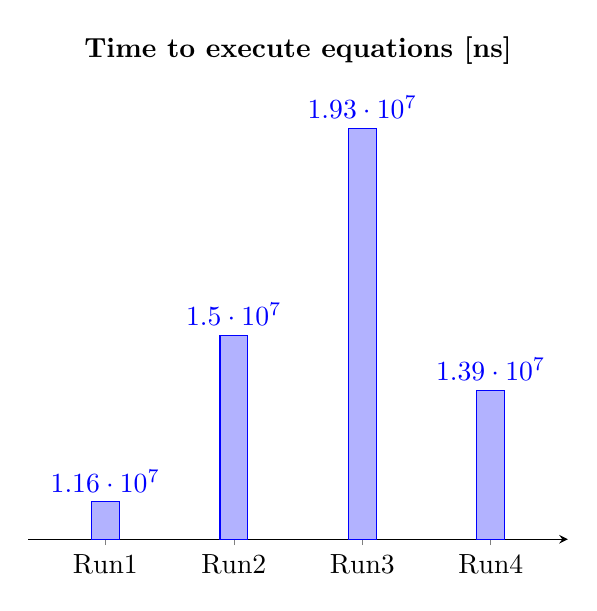
\begin{tikzpicture}
\begin{axis}[ybar, title={\textbf{Time to execute equations [ns]}}, symbolic x coords={Run1, Run2, Run3, Run4},
  legend pos = north west, axis y line=none, axis x line=bottom, nodes near coords, enlarge x limits=0.2, ] 
\addplot+ coordinates {(Run1, 
11558817
) (Run2, 
14991194
) (Run3, 
19259172
) (Run4, 
13859149
)}; 
\end{axis} 
\end{tikzpicture} 
\end{document}
